\documentclass[12pt, aspectratio=1610]{beamer}
\RequirePackage{
    amsmath,
    amssymb,
    calc,
    cancel,
    booktabs,
    color,
    siunitx,
    tikz,
    wrapfig,
    array,
    leftidx,
    float,
    etoolbox,
    fancyhdr,
    longtable,
    hyperref,
    ltcaption,
    ulem,
    wasysym,
    accents,
}

\sisetup{
    detect-all              = true,
    separate-uncertainty    = true,                                   % 7.2 ± 0.5
    multi-part-units        = single,
    per-mode                = reciprocal,                   % symbol for "m/s", reciprocal for "ms^{-1}"
    group-separator         = {\,},
    group-minimum-digits    = 5,
    inter-unit-product      = {\kern 0.10em},
    exponent-product        = \cdot,                        % \times for 5 × 10^7, \cdot for 5 . 1O^7    
    number-unit-product     = {\ },
    output-decimal-marker   = {\text{.}},
    range-units             = single,
    range-phrase            = {\text{ -- }},
    list-units              = single,
    list-final-separator    = {\text{\ a\ }},
    retain-explicit-plus    = true,
}

\hypersetup{
    hidelinks,
    breaklinks              = true,
}

\usepackage[
    final
]{pdfpages}

\usepackage[many]{tcolorbox}
\RenewDocumentCommand{\vec}{m}{\overrightarrow{#1}}

\makeatletter
    \def\new@mathgroup{\alloc@8\mathgroup\mathchardef\@cclvi}
    \patchcmd{\document@select@group}{\sixt@@n}{\@cclvi}{}{}
    \patchcmd{\select@group}{\sixt@@n}{\@cclvi}{}{}
\makeatother

\RequirePackage{mathspec}                                   % includes fontspec
\RequirePackage{polyglossia}                                % multi-language support
\RequirePackage{xunicode}
\setdefaultlanguage{slovak}

% Setup fonts -- see fontspec/mathspec documentation.
% Fonts are loaded from .ttf and .otf files in the core/fonts/ directory. We NEVER use system fonts.
\defaultfontfeatures{
    Mapping         = tex-text,
    Scale           = MatchLowercase,
    Ligatures       = TeX
}

\DeclareSIUnit\au{AU}
\DeclareSIUnit\pixel{px}
\DeclareSIUnit\lightyear{ly}
\DeclareSIUnit\parsec{pc}
\DeclareSIUnit\earthmass{M_{\earth}}
\DeclareSIUnit\speedoflight{c}
\DeclareSIUnit\foe{foe}
\DeclareSIUnit\year{yr}
\DeclareSIUnit\eur{€}
\DeclareSIUnit\solarmass{M_{\astrosun}}
\DeclareSIUnit\solarluminosity{L_{\astrosun}}
\DeclareSIUnit{\byte}{B}

\DeclareMathOperator{\diff}{\mathrm{d}\!}
\DeclareMathOperator{\pdiff}{\partial\!}

\NewDocumentCommand{\slashfrac}{m m}{\left.#1\middle/#2\right.}
\NewDocumentCommand{\derive}{O{} m m}{\frac{\mathop{\mathrm{d}^{#1}#2}}{\mathop{\mathrm{d}#3^{#1}}}}
%\NewDocumentCommand{\derive}{O{} m m}{\frac{\diffe^{#1}#2}{\diffe#3^{#1}}}
\NewDocumentCommand{\pderive}{O{} m m}{\frac{\partial^{#1} #2}{\partial #3^{#1}}}

\NewDocumentCommand{\integrate}{O{} O{} m m}{\int\limits_{#1}^{#2} \! #3 \, \diff#4}
\NewDocumentCommand{\iintegrate}{O{} O{} m m m}{\iint\limits_{#1}^{\quad#2} #3 \d#4\!\d#5}
\NewDocumentCommand{\iiintegrate}{O{} O{} m m m m}{\iiint\limits_{#1}^{\quad#2} #3 \d#4\!\d#5\!\d#6}

\NewDocumentCommand{\labelmath}{m +m}{%
    \begin{equation}%
        #2%
        \label{#1}%
    \end{equation}%
}

\NewDocumentCommand{\labelalign}{m +m}{%
    \begin{align}%
        #2%
        \label{#1}%
    \end{align}%
}

\linespread{1.0}
\setlength{\parindent}{0cm}
\setlength{\parskip}{6pt}
\setlength{\abovedisplayskip}{0mm}
\setlength{\belowdisplayskip}{0mm}
\setlength{\abovedisplayshortskip}{0mm}
\setlength{\belowdisplayshortskip}{0mm}
\setlength{\itemindent}{0pt}
\setlength{\textfloatsep}{0mm}
\setlength{\tabcolsep}{3mm}
\setlength{\LTcapwidth}{0.8\textwidth}
\renewcommand{\arraystretch}{1.2}

\setcounter{secnumdepth}{2}
\linespread{1.0}
\setlength{\parindent}{0cm}
\setlength{\parskip}{6pt}
\setlength{\abovedisplayskip}{0mm}
\setlength{\belowdisplayskip}{0mm}
\setlength{\abovedisplayshortskip}{0mm}
\setlength{\belowdisplayshortskip}{0mm}
\setlength{\itemindent}{0pt}
\setlength{\textfloatsep}{0mm}
\setlength{\tabcolsep}{3mm}
\renewcommand{\arraystretch}{1.2}

\setcounter{secnumdepth}{0}

\NewDocumentCommand{\fspicture}{m O{W} O{black}}{
    {
        \setbeamertemplate{navigation symbols}{}
        \setbeamercolor{background canvas}{bg = #3}
        \begin{frame}[plain]
            \begin{tikzpicture}[remember picture, overlay]
                \node[at=(current page.center)] {
                    \ifstrequal{H}{#2}{                                  
                        \includegraphics[height=\paperheight]{#1}%
                    }{%
                        \includegraphics[width=\paperwidth]{#1}%
                    }
                };
            \end{tikzpicture}
        \end{frame}
    }
}

\NewDocumentCommand{\frejm}{m +m}{
    \begin{frame}
        \frametitle{#1}
        #2
    \end{frame}
}
\defbeamertemplate{description item}{align center}{\hfill\insertdescriptionitem\hfill}
\definecolor{desc}{rgb}{0.66, 0, 0}
\definecolor{citem}{rgb}{0.72, 0, 0}
\definecolor{csitem}{rgb}{0.90, 0, 0}
\definecolor{cssitem}{rgb}{1, 0.1, 0.1}
\definecolor{qprimarybg}{rgb}{0.95, 0.95, 0.95}
\definecolor{check}{rgb}{0, 0.8, 0}

\setbeamertemplate{navigation symbols}{}
\newfontfamily{\semibold}{Segoe UI Semibold}
\RenewDocumentCommand{\emph}{m}{{\semibold#1}}

\mode<presentation> {
    \usetheme{Szeged}
    \usecolortheme{beaver}
    
    \usefonttheme{professionalfonts}
    \setallmainfonts{Minion Pro}
    \setmathrm{Minion Pro}
    
    \setsansfont{Segoe UI}
    \setmonofont{Consolas}
    \setbeamercolor*{enumerate item}{fg = citem}
    \setbeamercolor*{enumerate subitem}{fg = csitem}
    \setbeamercolor*{enumerate subsubitem}{fg = cssitem}
    \setbeamercolor*{description item}{fg = desc}
    \setbeamercolor*{itemize item}{fg = citem}
    \setbeamercolor*{itemize subitem}{fg = csitem}
    \setbeamercolor*{itemize subsubitem}{fg = cssitem}
    \setbeamercolor*{palette primary}{fg = red, bg = qprimarybg}
}

\AtBeginSection[]{
    \subsection{\insertsection}
    \begin{frame}
        \vfill
        \centering
        \begin{beamercolorbox}[sep = 8pt, center, shadow = true, rounded = true]{title}
            \usebeamerfont{title}\insertsectionhead\\[1.5mm]%
            \vfill
        \end{beamercolorbox}
        \vfill
    \end{frame}
}
\makeatletter

% Render percent sign with nice font, not ugly Computer modern
    \mathcode`\%="7025

% Fixes mathspec bug -- URL numbers are rendered with wrong font
    \ernewcommand\eu@MathPunctuation@symfont{Latin:m:n}
    \DeclareMathSymbol{,}{\mathpunct}{\eu@MathPunctuation@symfont}{`,}
    \DeclareMathSymbol{.}{\mathord}{\eu@MathPunctuation@symfont}{`.}
    \DeclareMathSymbol{<}{\mathrel}{\eu@MathPunctuation@symfont}{`<}
    \DeclareMathSymbol{>}{\mathrel}{\eu@MathPunctuation@symfont}{`>}
    \DeclareMathSymbol{/}{\mathord}{\eu@MathPunctuation@symfont}{`/}
    \DeclareMathSymbol{;}{\mathpunct}{\eu@MathPunctuation@symfont}{`;}
    \DeclareMathSymbol{(}{\mathopen}{\eu@DigitsArabic@symfont}{`(}
    \DeclareMathSymbol{)}{\mathclose}{\eu@DigitsArabic@symfont}{`)}
    \XeTeXDeclareMathSymbol{^^^^2026}{\mathinner}{\eu@MathPunctuation@symfont}{"2026}[\mathellipsis]
    \DeclareMathSymbol{0}{\mathalpha}{\eu@DigitsArabic@symfont}{`0}
    \DeclareMathSymbol{1}{\mathalpha}{\eu@DigitsArabic@symfont}{`1}
    \DeclareMathSymbol{2}{\mathalpha}{\eu@DigitsArabic@symfont}{`2}
    \DeclareMathSymbol{3}{\mathalpha}{\eu@DigitsArabic@symfont}{`3}
    \DeclareMathSymbol{4}{\mathalpha}{\eu@DigitsArabic@symfont}{`4}
    \DeclareMathSymbol{5}{\mathalpha}{\eu@DigitsArabic@symfont}{`5}
    \DeclareMathSymbol{6}{\mathalpha}{\eu@DigitsArabic@symfont}{`6}
    \DeclareMathSymbol{7}{\mathalpha}{\eu@DigitsArabic@symfont}{`7}
    \DeclareMathSymbol{8}{\mathalpha}{\eu@DigitsArabic@symfont}{`8}
    \DeclareMathSymbol{9}{\mathalpha}{\eu@DigitsArabic@symfont}{`9}
\makeatother


\usepackage{tabularx}


\title{The AMOS database system}
\subtitle{Storing data, one meteor at a time}
\author{Mgr. Martin Baláž}
\institute{DAA DAPEM colloquium}
\date{2019--04--17}

\begin{document}
    \begin{frame}
        \titlepage
    \end{frame}
                
    \section{Overview}
        \subsection{Overview}
            \frejm{Contents}{
                \setbeamersize{description width = 30mm}
                \begin{description}
                    \item[objective]        What are we doing?
                    \item[motivation]       Why?
                    \item[implementation]   How?
                    \item[results]          What have we done?
                \end{description}
            }
            
            \frejm{Objective}{
                \begin{itemize}
                    \item to build a database system for storing AMOS meteor data
                    \pause
                    \item and a simple dashboard for monitoring the network status
                    \pause 
                    \item it should be
                    \setbeamersize{description width = 40mm}
                    \begin{description}
                        \item<1->[web-based]        accessible from anywhere
                        \item<2->[comprehensible]   we are able to identify interesting events easily
                        \item<3->[autonomous]       integrate the entire processing pipeline
                    \end{description}
                \end{itemize}
            }
            
            \frejm{Motivation}{
                Current state is \only<1>{a disaster}\only<2->{\sout{a disaster} slightly suboptimal}
                \pause
                \begin{itemize}
                    \item no unified data file format
                    \item data spread across multiple computers
                    \item analysis next to impossible
                    \begin{itemize}
                        \item and I badly missed it in my diploma thesis
                    \end{itemize}
                \end{itemize}
                \pause
                \emph{Let us tidy up and organize the data!}
            }
        
    \section{Data}
        \subsection{Data}
            \frejm{Acquisition}{
                Data are acquired by AMOS cameras
                \begin{itemize}
                    \item \emph{UFOCapture} by SonotaCo
                    \item \emph{AMOS} by Kvant
                    \begin{itemize}
                        \item will be ready in about two months...
                        \pause
                        \item ...for the last three years
                    \end{itemize}
                \end{itemize}
            }
            
            \frejm{Pre-processing}{
                First of all, raw data are filtered and annotated

                \begin{itemize}
                    \item meteor recognition and data extraction
                    \begin{itemize}
                        \item position in the sky
                        \item magnitude
                        \item angular speed
                        \item ...
                    \end{itemize}
                    \pause
                    \item saved in an \code{XML} file
                    \item raw video stored in uncompressed \code{AVI} file
                    \item overview in a \code{JPG} file
                \end{itemize}
                \pause
                \begin{itemize}
                    \item not much can be easily done about this
                \end{itemize}
            }
            
            \frejm{Retrieval}{
                \emph{Currently}:
                \begin{itemize}
                    \item UFOCapture launches a \code{bat} file
                    \item mail transfer via SMTP (e-mail)
                    \item processed by \code{charon}
                \end{itemize}
                \pause
                \emph{Proposal}:
                \begin{itemize}
                    \item video capturing software forwards data to a daemon
                    \item sent over HTTP in a POST request
                \end{itemize}
            }

            \frejm{Retrieval -- proposed approach}{
                We may need an \emph{API}
                \begin{itemize}
                    \item station submits a new \model{Sighting}
                    \item website retrieves a list of \model{Meteor}s
                    \item daemon periodically computes \model{Meteor} data
                    \item data exports
                    \begin{itemize}
                        \item scientific analyses
                        \item maps (with JavaScript)
                        \item integration with other services
                    \end{itemize}
                \end{itemize}
            }
            
            \frejm{Processing}{
                Data need to be \emph{validated} and \emph{processed}
                \begin{itemize}
                    \item remove invalid data (false detections, ...)
                    \item compute actual meteor positions from multiple sightings
                    \begin{itemize}
                        \item currently done by \code{MT}
                        \item only use its output
                        \item write import routines
                    \end{itemize}
                \end{itemize}
            }
            
            \frejm{Storage}{
                At this point the data are ready to be stored
                \begin{itemize}
                    \item in a \emph{structured} and \emph{semantic} way
                    \item consistency is \emph{enforced} at all times
                    \item auxiliary data
                    \begin{itemize}
                        \item housekeeping
                        \item statistics
                    \end{itemize}
                \end{itemize}
            }

            \frejm{Data retention}{
                To prevent problems down the line, we should
                \pause
                \begin{itemize}
                    \item keep \emph{all} raw data available
                    \pause
                    \item \emph{never} delete anything
                    \begin{itemize}
                        \item unless provably \emph{incorrect}
                    \end{itemize}
                    \pause
                    \item enable raw data re-processing
                    \begin{itemize}
                        \item data import from an offline station                        
                        \item manual correction
                        \item new processing algorithms
                    \end{itemize}
                \end{itemize}
            }

            \frejm{Housekeeping}{
                \textit{Def:} Data of \emph{low scientific value} but \emph{high operational importance}\\[10mm]
                \pause
                \begin{columns}
                    \begin{column}{0.33\textwidth}
                        \begin{itemize}
                            \item environment
                                \begin{itemize}
                                    \item temperature
                                    \item humidity
                                    \item pressure
                                    \item ...
                                \end{itemize}
                        \end{itemize}
                    \end{column}
                    \begin{column}{0.33\textwidth}
                        \begin{itemize}
                            \item station
                                \begin{itemize}
                                    \item system uptime
                                    \item UPS status
                                    \item disk usage
                                    \item ...
                                \end{itemize}
                        \end{itemize}
                    \end{column}
                    \begin{column}{0.33\textwidth}
                        \begin{itemize}
                            \item network
                                \begin{itemize}
                                    \item connection
                                    \item IP address
                                    \item last data
                                    \item ...
                                \end{itemize}
                        \end{itemize}
                    \end{column}
                \end{columns}
                \pause
                \vspace{8mm}
                Everything is displayed on a \emph{dashboard}
            }
        
    \section{Database}
        \subsection{Database}
            \frejm{The database}{
                \emph{Problem}: We need a way to visualize and comprehend the data

                \pause
                \emph{Solution}: A database and a simple web interface
                \begin{itemize}
                    \item provides a basic framework for data operations
                    \item much more user-friendly than a bare directory listing
                    \item much easier to retrieve, sort and analyze the data
                \end{itemize}
            }

            \frejm{Design}{
                Underlying data are well-structured and suitable for an \emph{object-relational} database
            
                \begin{itemize}
                    \item ORDBMS
                    \begin{itemize}
                        \item data are stored in \emph{relations} (tables)
                        \item each column stores the same \emph{property}
                        \item each row stores a single \emph{entity} (object)
                        \item each object has an identifier -- \emph{primary key}
                        \item fields may point to other tables -- \emph{foreign keys}
                        \item data are accessed and manipulated using a \emph{query language}
                    \end{itemize}
                \end{itemize}
            }

            \begin{frame}[fragile]
                \frametitle{ORDBMS}
                \small
                \begin{overlayarea}{\textwidth}{0.7 \textheight}
                    \ \\
                    \highlightbox<2>{orange}{\texttt{SELECT "id", "timestamp", "magnitude" \textbackslash}} \\
                    \highlightbox<3>{orange}{\texttt{FROM "meteors" \textbackslash}} \\
                    \highlightbox<4>{orange}{\texttt{WHERE "timestamp" BETWEEN "2019-04-16 15:00:00" AND "2019-04-17 09:00:00" \textbackslash}} \\
                    \highlightbox<5>{orange}{\texttt{ORDER BY "magnitude" ASC \textbackslash}} \\
                    \highlightbox<6>{orange}{\texttt{LIMIT 5;}}
                    \vspace{5mm}
                    \begin{onlyenv}<7>
                    \begin{verbatim}
356, "2019-04-17 03:45:10", -5.8
728, "2019-04-17 04:14:23", -3.2
456, "2019-04-16 23:56:04", -2.7
908, "2019-04-17 01:23:45", -2.5
854, "2019-04-16 21:58:35", -2.2
                    \end{verbatim}
                    \end{onlyenv}
                \end{overlayarea}
            \end{frame}
                    
            \frejm{Models}{
                The art and science of creating databases...

                \pause
                ...is to naturally translate the real world to models:
                \pause
                \begin{itemize}
                    \item \model{Meteor}
                    \item \model{Sighting}
                    \item \model{Station}
                    \item \model{Subnetwork}
                    \item \model{Country}
                    \item ...more as needed
                \end{itemize}
            }
            
            \frejm{Model \model{Sighting}}{
                Describes the \emph{sighting} of a single meteor by an AMOS camera
                \pause
                \begin{itemize}    
                    \item identifier
                    \item observed projected position on the sky
                        \item three coordinates
                        \begin{itemize}
                            \item azimuth
                            \item altitude
                        \end{itemize}
                        \pause
                        \item at three moments
                        \begin{itemize}
                            \item \emph{beginning}
                            \item \emph{maximum brightness}
                            \item \emph{end}
                        \end{itemize}      
                    \item maximum apparent magnitude            
                \end{itemize}
            }
            
            \frejm{Model \model{Sighting} -- extras}{
                \begin{itemize}
                    \item miscellaneous computed information
                        \begin{itemize}
                            \item arc length
                            \item duration
                            \item Sun and Moon info
                            \begin{itemize}
                                \item position
                                \item elongation
                                \item magnitude
                                \item not stored in the database
                            \end{itemize}
                        \end{itemize}
                    \pause
                    \item visualisation
                        \begin{itemize}
                            \item real photograph from AMOS
                            \item corresponding simulation (?)
                        \end{itemize}                    
                \end{itemize}
            }
            
            \frejm{Model \model{Meteor}}{  
                Describes the actual \emph{event}, an atmospheric entry of a meteoroid particle
                \begin{itemize}
                    \item \emph{timestamp}
                    \item true geographic location
                    \begin{itemize}
                        \item again, four coordinates
                        \begin{itemize}
                            \item \emph{timestamp}
                            \item \emph{latitude}
                            \item \emph{longitude}
                            \item \emph{altitude}
                        \end{itemize}
                        \pause
                        \item at three moments
                        \begin{itemize}
                            \item \emph{beginning}
                            \item \emph{maximum brightness}
                            \item \emph{end}
                        \end{itemize}
                    \end{itemize}
                \end{itemize}
            }
            
            \frejm{Model \model{Meteor} -- auxiliary data}{
                \begin{itemize}                
                    \item true \emph{trail length}
                    \begin{itemize}
                        \item this is not well-defined
                    \end{itemize}
                    \item computed maximal \emph{absolute magnitude} (least-squares)
                    \item \emph{visualisation}
                    \begin{itemize}
                        \item \code{KML} file for \emph{Google Earth}
                        \item \emph{online map} (OpenLayers)
                    \end{itemize}
                \end{itemize}
            }
        
            \frejm{Database diagram}{
                \includegraphics[page = 2, width = 0.875 \textwidth]{diagram.pdf}
            }
    
    \section{Visualisation}
        \subsection{Visualisation}
            \frejm{Overview}{
                We have implemented a website in \emph{Python/Django}

                \begin{itemize}
                    \item webserver + CRUD operations
                    \item administration interface (courtesy of Django)
                    \item REST framework
                \end{itemize}
            }

            \frejm{Dashboard}{
                We need to detect problems and bring them to attention
                \pause
                \begin{itemize}
                    \item add \code{status} to \model{Station}
                    \item various problems can be detected and addressed
                    \begin{itemize}
                        \item lost connection
                        \item lost power
                        \item software problems
                        \item AMOS hardware failure
                        \item no data
                        \item ...
                    \end{itemize}
                    \pause
                    \item requires station-side changes to software
                \end{itemize}
            }

            \frejm{System in operation}{
                As of now, the core of the system is operational
                \begin{itemize}
                    \item \href{http://192.168.0.177:4805/}{dashboard}
                    \item \href{http://192.168.0.177:4805/meteors/}{meteor list}
                    \item \href{http://192.168.0.177:4805/sighting/2537}{example of a sighting}
                    \item \href{http://192.168.0.177:4805/meteor/example/path}{example of a meteor path}
                \end{itemize}                 
                \pause
                We need to implement
                \begin{itemize}
                    \item remote station monitoring
                    \item data import routines
                    \item data export (\code{CSV}, \code{JSON}, ...)
                    \item API
                \end{itemize}
            }

            \frejm{And then?}{
                The system will enable us to do much more:
                \begin{columns}
                    \begin{column}{0.6\textwidth}
                        \begin{itemize}
                            \item sort and display meteors by any criteria
                            \pause
                            \item display meteor activity
                            \item use data from \code{Asmodeus} to estimate flux
                            \pause
                            \item provide foundation for my PhD thesis
                            \pause
                            \item provide data for \emph{you}
                        \end{itemize}
                    \end{column}
                    \begin{column}{0.3\textwidth}
                        
\includegraphics[width = \linewidth]{unclesam.jpg}
                    \end{column}
                \end{columns}
            }
    
        \frejm{Thank you for your attention}{
            {\large \textit{Above all else, show the data.}}
            \scriptsize
            \begin{flushright}
                Edward R. Tufte\\
                The Visual Display of Quantitative Information, 1983
            \end{flushright}
        }      
                
        \frejm{References}{
            \begin{itemize}
                \item \textbf{Database.Guide}:
                    What is an ORDBMS? \texttt{https://database.guide/what-is-an-ordbms/}
                \item \textbf{James Montgomery Flagg}:
                    Uncle Sam Needs You (US Propaganda material). 1917.
                \item \textbf{holistics.io}:
                    \texttt{dbdiagram.io} database relationship diagram tool. \texttt{https://dbdiagram.io/}.
            \end{itemize}
        }
            
\end{document}
